\documentclass[11pt]{article}
\usepackage[letterpaper,margin=.78in,headheight=15pt]{geometry}
\usepackage[T1]{fontenc}
\usepackage[utf8]{inputenc}
\usepackage{lmodern,microtype,amsmath,amssymb,graphicx,xcolor,fancyhdr,hyperref,booktabs,array}
\usepackage{tcolorbox}
\definecolor{navy}{HTML}{17334D}
\definecolor{teal}{HTML}{168B8D}
\definecolor{pale}{HTML}{F2F7F8}
\hypersetup{colorlinks=true,linkcolor=teal,urlcolor=teal,pdftitle={Quadratic-Form Engine / K-COS: Visual Guide},pdfauthor={Komorebi P.}}
\pagestyle{fancy}\fancyhf{}
\fancyhead[L]{\small\color{navy}Quadratic-Form Engine / K-COS}
\fancyhead[R]{\small\color{navy}Visual Guide}
\fancyfoot[L]{\small\color{navy}Komorebi P.\quad October 7, 2026}
\fancyfoot[R]{\small\color{navy}\thepage}
\renewcommand{\headrulewidth}{.4pt}
\setlength{\parindent}{0pt}\setlength{\parskip}{7pt}
\setlength{\emergencystretch}{2em}
\setlength{\abovedisplayskip}{7pt}\setlength{\belowdisplayskip}{7pt}
\begin{document}
{\small\bfseries\color{teal}Quadratic-Form Engine / K-COS \textperiodcentered{} Visual companion \textperiodcentered{} Final edition}

{\LARGE\bfseries\color{navy}From a large factor to a justified tail\par}
\vspace{3pt}
\begin{center}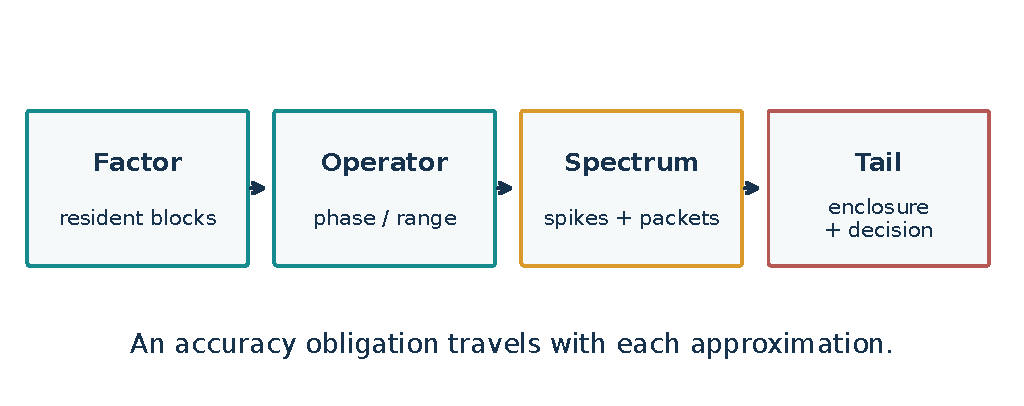
\includegraphics[width=\linewidth,height=3.1in,keepaspectratio]{figures/00_pipeline.pdf}\end{center}
{\small\color{navy}The four representation layers are compatible, but their accuracy obligations remain distinct.}

The engine connects a replayable matrix factor to a Gaussian quadratic-form probability. Its successive representations answer different questions: which data must reside in memory, which operator blocks can propagate, which range remains unresolved, and which transform approximation can meet the requested accuracy.

This guide develops that connection through small declared models. Integer checks verify the block identities and exact phase zeros. Floating plots illustrate spectra, packet remainders, and cosine decay. A positive finite-sum control gives a logarithmic view of deep tails. None of these figures is a new production benchmark.

Read the traditional paper for complete proofs and the Lean guide for the formalization inventory and checked build scope. The final page identifies the boundary between algebraic identities, analytic bounds, and an executable numerical enclosure.

\begin{tcolorbox}[colback=pale,colframe=teal,boxrule=.4pt,arc=2pt,left=7pt,right=7pt,top=5pt,bottom=5pt]\small\bfseries Preserve exact identities where possible. Expose every approximation at the point where it enters.\end{tcolorbox}
\vfill{\footnotesize\color{navy}\textbf{Source anchors.} Traditional paper: Decomposition axes; Weighted-feature specialization.}
\clearpage
{\small\bfseries\color{teal}01 \textperiodcentered{} Factor and law}

{\LARGE\bfseries\color{navy}A spectrum is the distributional interface\par}
\vspace{3pt}
\begin{center}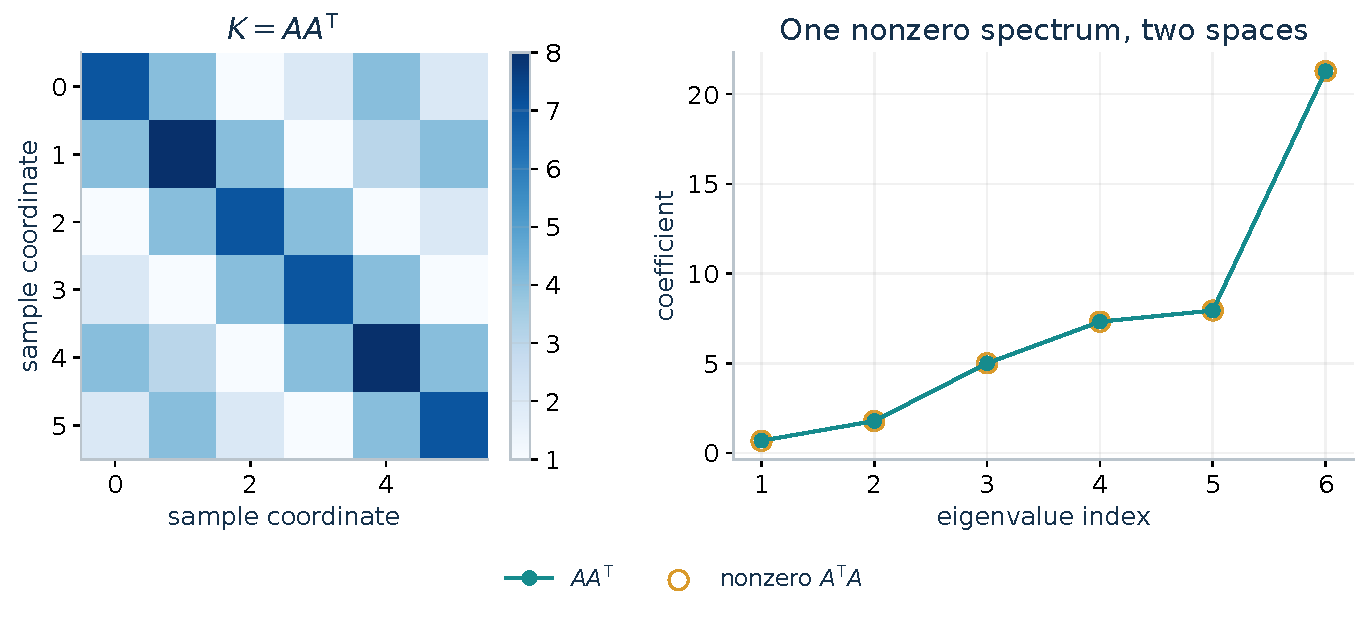
\includegraphics[width=\linewidth,height=3.1in,keepaspectratio]{figures/01_factor_spectrum.pdf}\end{center}
{\small\color{navy}A declared integer factor, shown through its kernel and two numerically evaluated nonzero spectra.}

\[X=\Sigma^{1/2}Z,\quad Z\sim N(0,I),\quad H=\Sigma^{1/2}M\Sigma^{1/2}.\]
\[X^{\mathsf T}MX\overset d=\sum_{j=1}^{r}\lambda_jZ_j^2,\qquad \lambda_j\in\operatorname{spec}(H)\setminus\{0\}.\]
For a central Gaussian vector with covariance $\Sigma\succeq0$ and symmetric $M$, the quadratic form becomes a weighted sum of independent standard-normal squares after whitening and orthogonal diagonalization. The operator may originate in a kernel, a signal model, or another symmetric construction. Once its spectrum has been correctly obtained, the tail layer sees those coefficients.

The nonzero eigenvalues of the two Gram matrices coincide. The small integer factor in this guide has six sample coordinates and nine feature coordinates. One Gram matrix therefore has six eigenvalues; the other has the same six nonzero eigenvalues plus three zeros. The figure compares their floating evaluations.

Positive coefficients give support on the nonnegative half-line. Signed coefficients define a different support problem. The exact reduction extends to symmetric indefinite forms, while the positive-support interval backend developed later has narrower hypotheses.

\begin{tcolorbox}[colback=pale,colframe=teal,boxrule=.4pt,arc=2pt,left=7pt,right=7pt,top=5pt,bottom=5pt]\small\bfseries Representation equivalence is exact mathematics. Certifying computed eigenvalues is a further numerical obligation.\end{tcolorbox}
\vfill{\footnotesize\color{navy}\textbf{Source anchors.} Traditional paper: General quadratic-form core / Representation equivalence; Exact central signed reduction.}
\clearpage
{\small\bfseries\color{teal}02 \textperiodcentered{} Storage partition}

{\LARGE\bfseries\color{navy}Column blocks add their Gram operators exactly\par}
\vspace{3pt}
\begin{center}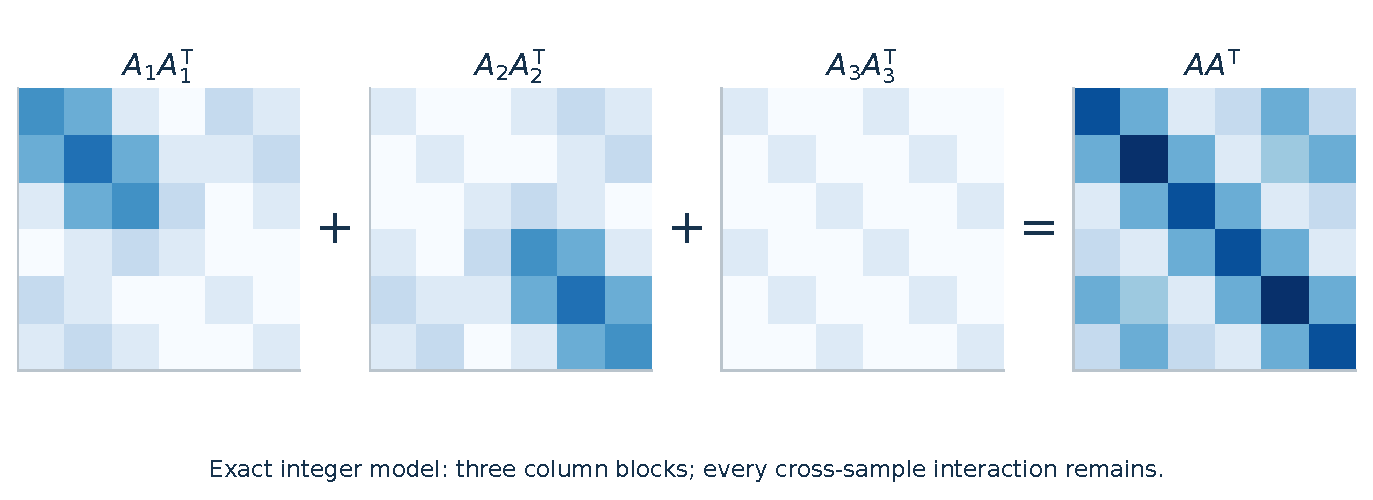
\includegraphics[width=\linewidth,height=3.1in,keepaspectratio]{figures/02_block_gram.pdf}\end{center}
{\small\color{navy}All block Gram contributions use the same color scale. Their exact sum is the full sample kernel.}

\[A=[A_1\ \cdots\ A_B],\qquad AA^{\mathsf T}=\sum_{b=1}^B A_bA_b^{\mathsf T}.\]
\[KV=\sum_b A_b(A_b^{\mathsf T}V),\qquad A_b\in\mathbb R^{n\times c_b},\quad V\in\mathbb R^{n\times s}.\]
Partition a factor by columns and keep every block. Horizontal concatenation turns the sample-space Gram matrix into a sum of block Gram matrices. Changing the block widths or the order in which blocks are read preserves the represented operator.

The figure splits the declared $6\times9$ integer factor into three blocks of width three. Every matrix entry in the displayed identity is an integer, and the regeneration script checks equality exactly. Block storage introduces no statistical approximation.

A streamed action need not store each block kernel. It first multiplies by the block transpose, then by the block itself, and accumulates the sample-space result. The dimensions explain why the operator can remain exact even when the whole factor cannot reside at once.

\begin{tcolorbox}[colback=pale,colframe=teal,boxrule=.4pt,arc=2pt,left=7pt,right=7pt,top=5pt,bottom=5pt]\small\bfseries Execution partitions determine residence and I/O. Keeping all blocks preserves the operator.\end{tcolorbox}
\vfill{\footnotesize\color{navy}\textbf{Source anchors.} Traditional paper: Variant-block Gram decomposition; Exact streamed kernel actions.}
\clearpage
{\small\bfseries\color{teal}03 \textperiodcentered{} Algebraic sizing}

{\LARGE\bfseries\color{navy}Memory depends on the resident width\par}
\vspace{3pt}
\begin{center}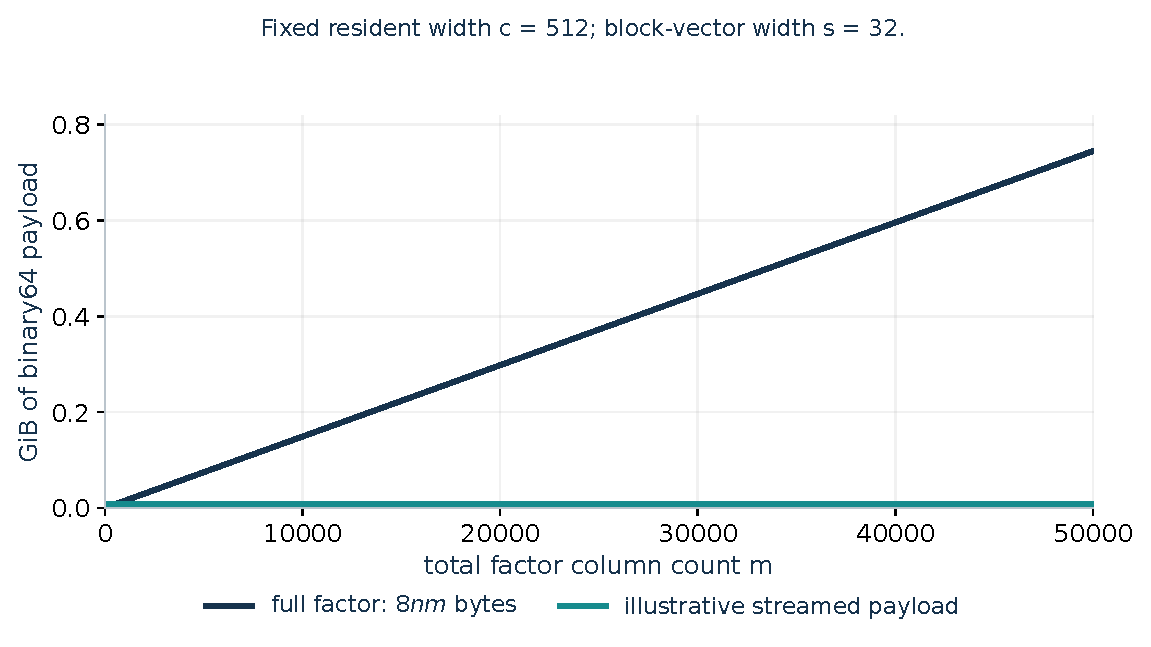
\includegraphics[width=\linewidth,height=3.1in,keepaspectratio]{figures/03_memory.pdf}\end{center}
{\small\color{navy}An explicitly counted binary64 payload with fixed resident width. Total-factor storage grows linearly in $m$.}

\[\text{working storage}=O(nc+ns+cs+np).\]
\[\text{illustrated payload}=8\,(nc+2ns+cs+np)\ \text{bytes}.\]
A full factor holds $nm$ scalar entries. A streamed action with resident width $c$ and block-vector width $s$ keeps a factor block and a small number of action buffers. Residualization against a covariate basis of rank $p$ adds $np$ entries. At fixed $c,s,p$, this algebraic working set does not grow with total column count $m$.

The sizing curve is an illustration, not a measured memory profile. It uses $n=2000$, $c=512$, $s=32$, $p=3$, and binary64 entries. The plotted streamed payload counts one resident factor, two sample buffers, one block intermediate, and the covariate basis.

Backend workspace, I/O buffers, saved outputs, and spectral-solver storage require their own accounting. A two-dimensional sample/feature tile also needs its tile-local covariate data. An algebraic storage bound does not promise a device-specific allocation total.

\begin{tcolorbox}[colback=pale,colframe=teal,boxrule=.4pt,arc=2pt,left=7pt,right=7pt,top=5pt,bottom=5pt]\small\bfseries Separate algebraic payload, implementation workspace, and persistent output when planning memory.\end{tcolorbox}
\vfill{\footnotesize\color{navy}\textbf{Source anchors.} Traditional paper: Exact streamed kernel actions / Working memory independent of total variant count; Two-dimensional sample/variant tiling.}
\clearpage
{\small\bfseries\color{teal}04 \textperiodcentered{} Weighted-feature specialization}

{\LARGE\bfseries\color{navy}Residualization is an orthogonal projection\par}
\vspace{3pt}
\begin{center}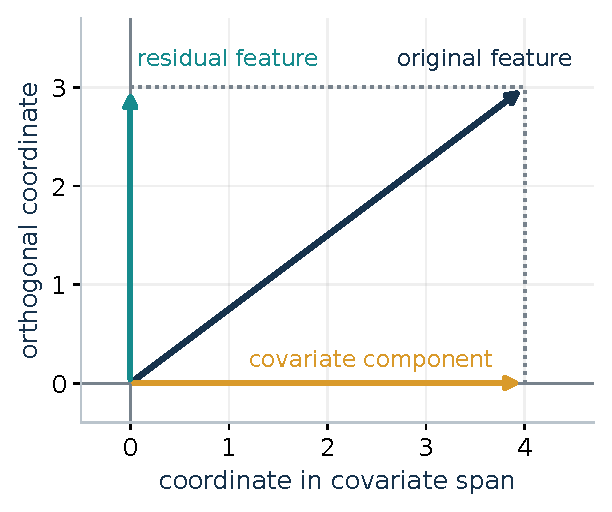
\includegraphics[width=\linewidth,height=3.1in,keepaspectratio]{figures/04_residualization.pdf}\end{center}
{\small\color{navy}An exact two-coordinate projection splits a feature into removed and retained components.}

\[Q_X^{\mathsf T}Q_X=I,\quad M_X=I-Q_XQ_X^{\mathsf T},\quad M_X^2=M_X=M_X^{\mathsf T}.\]
\[A=M_XGW^{1/2},\qquad K=AA^{\mathsf T}.\]
For a covariate range basis $Q_X$ with orthonormal columns, the residualizer $M_X=I-Q_XQ_X^{\mathsf T}$ removes the component in the covariate span. It is symmetric and idempotent. Applying it to the weighted feature factor restricts the kernel to variation left after the null-model covariates have been removed.

The two-coordinate control draws the exact split $(4,3)=(4,0)+(0,3)$. The horizontal axis represents the covariate span and the vertical axis its orthogonal complement. This picture explains the geometry; the general projector acts in the full sample space.

The factor $A=M_XGW^{1/2}$ is one specialization of the domain-independent engine. A correct range basis must represent the actual covariate span. Rank deficiency cannot be handled by silently treating extra QR columns as covariate directions.

\begin{tcolorbox}[colback=pale,colframe=teal,boxrule=.4pt,arc=2pt,left=7pt,right=7pt,top=5pt,bottom=5pt]\small\bfseries The general engine operates on factors. Residualized weighted features provide one important factor construction.\end{tcolorbox}
\vfill{\footnotesize\color{navy}\textbf{Source anchors.} Traditional paper: Weighted-feature specialization; Streaming directly from raw genotype blocks.}
\clearpage
{\small\bfseries\color{teal}05 \textperiodcentered{} Structural locality}

{\LARGE\bfseries\color{navy}Exact zeros create a finite phase cone\par}
\vspace{3pt}
\begin{center}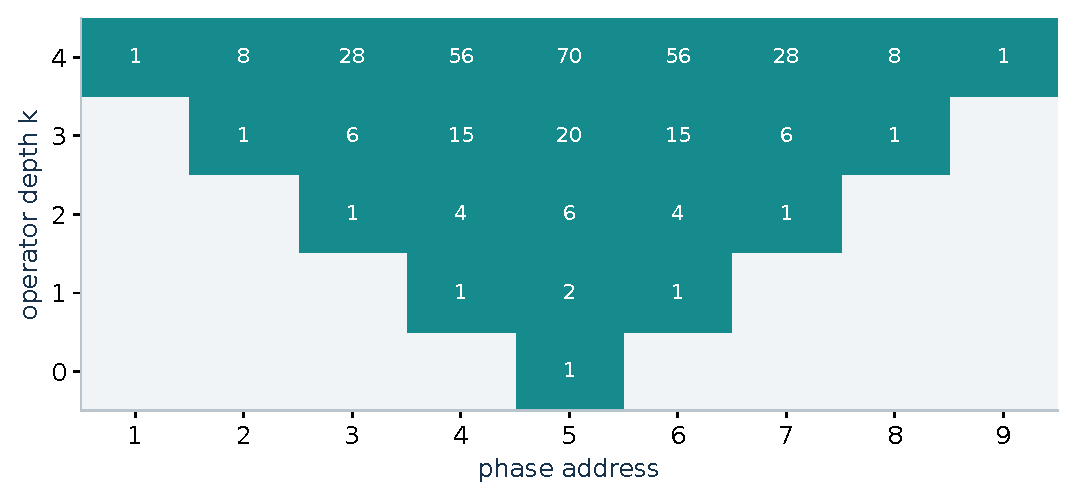
\includegraphics[width=\linewidth,height=3.1in,keepaspectratio]{figures/05_phase_cone.pdf}\end{center}
{\small\color{navy}Exact integer phase support for depths zero through four. A colored entry is genuinely nonzero.}

\[\sum_hP_h=I,\qquad g\to h\iff P_hHP_g\ne0.\]
\[\operatorname{dist}(g,h)>k\quad\Longrightarrow\quad P_hH^kP_g=0.\]
Choose a complete orthogonal family of phase projectors on feature space and form $H=A^{\mathsf T}A$. An edge from phase $g$ to phase $h$ exists when the transfer block $P_hHP_g$ is nonzero. Each operator application follows one graph edge; an iterate of depth $k$ cannot reach a phase farther than $k$ edges away.

The finite control is a nine-phase chain with $H=2I+S+S^{\mathsf T}$ and a unit start in phase five. The printed entries are exact integers in $H^kx$, and the shaded support expands by one phase at each step. The script checks every zero outside the cone.

These exact zeros justify omitting inactive phases for that finite-depth query. Storage blocks may still subdivide each active phase arbitrarily. The phase graph answers propagation questions, while the storage partition answers residence questions.

\begin{tcolorbox}[colback=pale,colframe=teal,boxrule=.4pt,arc=2pt,left=7pt,right=7pt,top=5pt,bottom=5pt]\small\bfseries A certified zero allows exact omission. A merely small coupling needs an error bound.\end{tcolorbox}
\vfill{\footnotesize\color{navy}\textbf{Source anchors.} Traditional paper: Polyphase structure / Polyphase light cone; Streaming-polyphase composition.}
\clearpage
{\small\bfseries\color{teal}06 \textperiodcentered{} Approximate locality}

{\LARGE\bfseries\color{navy}Weak edges need a transfer envelope\par}
\vspace{3pt}
\begin{center}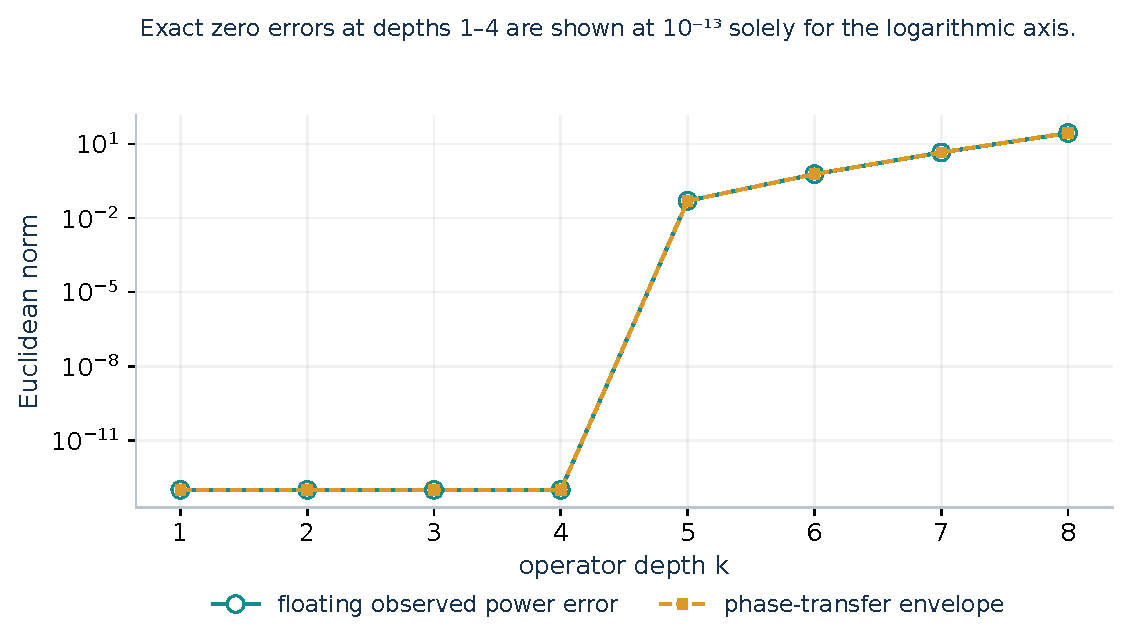
\includegraphics[width=\linewidth,height=3.1in,keepaspectratio]{figures/06_approximate_cone.pdf}\end{center}
{\small\color{navy}One declared weak-edge control. Exact zeros are plotted at a floor solely to fit the logarithmic axis.}

\[\rho(X)_h=\|P_hX\|_F,\qquad \mathcal B_{hg}=\|P_hHP_g\|_2.\]
\[\rho(H^kX)\le\mathcal B^k\rho(X),\qquad\rho((H^k-H_0^k)X)\le(\mathcal B^k-\mathcal B_0^k)\rho(X).\]
A weak nonzero coupling destroys the exact-zero conclusion. Record the spectral norm of every phase block in a nonnegative transfer matrix $\mathcal B$. The phase-norm profile of any block vector is dominated componentwise by multiplication with $\mathcal B$.

For a retained operator $H_0$, let $\mathcal B_0$ keep the corresponding entries. Telescoping the two operator powers gives a phasewise bound on the omitted action. Symmetric block retention preserves self-adjointness; the power estimate itself does not require the retained operator to be positive.

The toy chain receives a signed weak edge of weight $-0.035$ between phases one and nine. Starting in phase five, that edge has no effect through depth four. At later depths the figure compares floating observed error with the transfer-envelope evaluation. The theorem supplies the general bound; the plot checks this finite instance.

\begin{tcolorbox}[colback=pale,colframe=teal,boxrule=.4pt,arc=2pt,left=7pt,right=7pt,top=5pt,bottom=5pt]\small\bfseries Approximate locality produces a budgeted leakage quantity, not an exact support assertion.\end{tcolorbox}
\vfill{\footnotesize\color{navy}\textbf{Source anchors.} Traditional paper: Certified approximate light cones / Weighted phase-transfer envelope; Thresholded-power certificate.}
\clearpage
{\small\bfseries\color{teal}07 \textperiodcentered{} Core and residual}

{\LARGE\bfseries\color{navy}The unresolved range has positive structure\par}
\vspace{3pt}
\begin{center}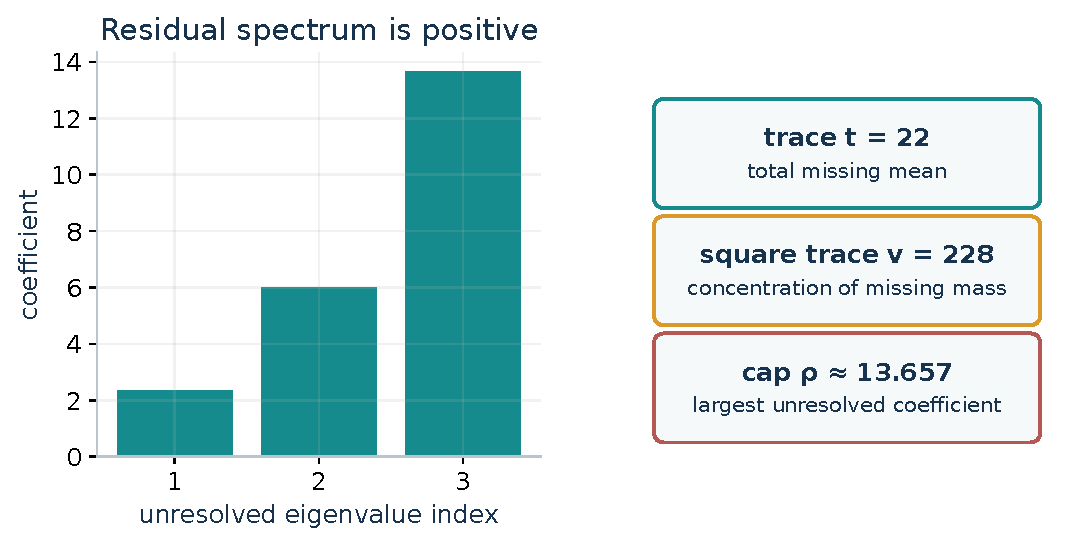
\includegraphics[width=\linewidth,height=3.1in,keepaspectratio]{figures/07_residual.pdf}\end{center}
{\small\color{navy}Positive residual coefficients and their invariants for a declared coordinate-range control.}

\[A=UB+F,\quad U^{\mathsf T}F=0,\quad A^{\mathsf T}A=B^{\mathsf T}B+F^{\mathsf T}F.\]
\[t=\operatorname{tr}R=\|F\|_F^2,\quad v=\operatorname{tr}(R^2),\quad \rho_R=\|R\|_2.\]
Let $U$ contain $d$ orthonormal sample-space directions. Project the factor into its captured range coordinates $B=U^{\mathsf T}A$ and residual $F=(I-UU^{\mathsf T})A$. Orthogonality eliminates the cross terms in the feature-space Gram matrix.

The missing term is the positive operator $R=F^{\mathsf T}F$. Its trace is the missing mean of the Gaussian quadratic form. Its square trace measures concentration, and its spectral norm caps any unresolved coefficient. These invariants convey more information than one generic operator-norm error.

The control captures the first three coordinate directions of the integer factor. Its Gram decomposition is checked exactly. Residual eigenvalues and the cap are floating diagnostics. A small residual norm alone does not prove that an extreme-tail probability has the requested relative accuracy.

\begin{tcolorbox}[colback=pale,colframe=teal,boxrule=.4pt,arc=2pt,left=7pt,right=7pt,top=5pt,bottom=5pt]\small\bfseries Unresolved spectral mass is an explicit object with its own trace, concentration, and cap.\end{tcolorbox}
\vfill{\footnotesize\color{navy}\textbf{Source anchors.} Traditional paper: Trace-aware residual certification and exact completion / Exact core--residual decomposition.}
\clearpage
{\small\bfseries\color{teal}08 \textperiodcentered{} Exact completion}

{\LARGE\bfseries\color{navy}A small remaining range can be completed\par}
\vspace{3pt}
\begin{center}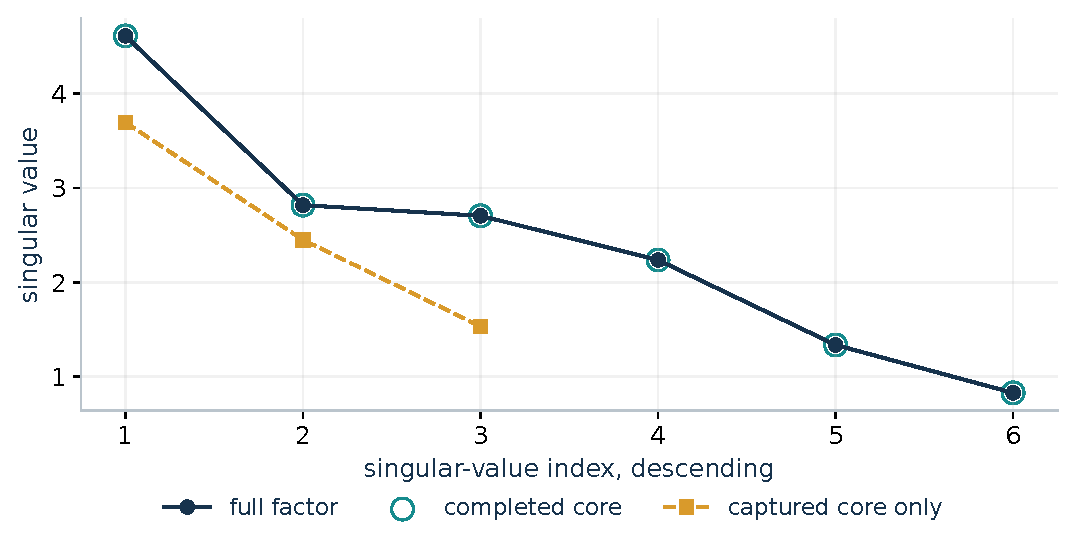
\includegraphics[width=\linewidth,height=3.1in,keepaspectratio]{figures/08_completion.pdf}\end{center}
{\small\color{navy}Completed and full singular spectra coincide in the integer factor control; the captured core is incomplete.}

\[U^{\mathsf T}W=0,\qquad A=[U\ W]\begin{bmatrix}B\\D\end{bmatrix}.\]
\[\left\lceil\max\{t/\rho_R,t^2/v\}\right\rceil\le\operatorname{rank}F\le n-d\quad(F\ne0).\]
If the residual admits $F=WD$ with orthonormal columns of $W$, its range lies orthogonal to $U$. Appending $W$ therefore creates an orthonormal synthesis factor, and stacking the two coordinate cores recovers the full factor.

The nonzero singular values of the completed core equal those of the original factor. The figure compares the incomplete captured core with the completed core in the declared integer example. Exact reconstruction of that factor is checked before numerical singular values are plotted.

Residual moments also provide a rank lower bound. Together with the orthogonal-complement dimension they can identify the missing rank when the two integers agree. A completion procedure must retain all genuine residual directions. A floating rank threshold has a separate error obligation.

\begin{tcolorbox}[colback=pale,colframe=teal,boxrule=.4pt,arc=2pt,left=7pt,right=7pt,top=5pt,bottom=5pt]\small\bfseries When the remaining rank is affordable, exact completion can replace further approximate iteration.\end{tcolorbox}
\vfill{\footnotesize\color{navy}\textbf{Source anchors.} Traditional paper: Trace-aware residual certification and exact completion / Residual-rank bracket; Exact residual completion.}
\clearpage
{\small\bfseries\color{teal}09 \textperiodcentered{} Probability reweighting}

{\LARGE\bfseries\color{navy}Tilting moves the query into the bulk\par}
\vspace{3pt}
\begin{center}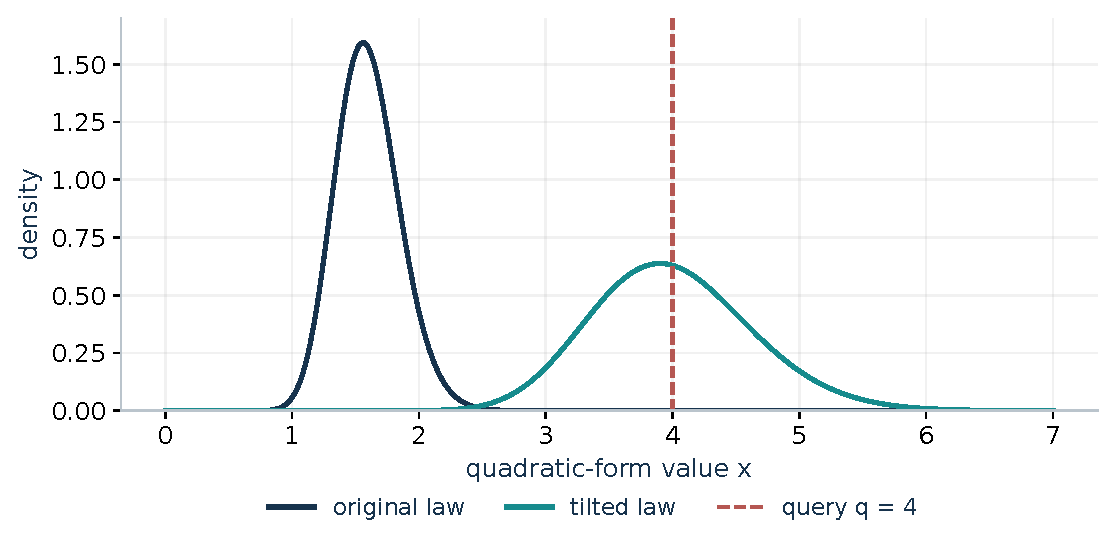
\includegraphics[width=\linewidth,height=3.1in,keepaspectratio]{figures/09_tilt.pdf}\end{center}
{\small\color{navy}The threshold becomes central under the tilted law. The likelihood-ratio weight restores the original tail.}

\[\kappa(s)=-\frac12\sum_j\log(1-2s\lambda_j),\qquad 0<\theta<\frac1{2\lambda_{\max}}.\]
\[P(Q\ge q)=e^{\kappa(\theta)-\theta q}\,\mathbb E_\theta[e^{-\theta(Q-q)}\mathbf1_{\{Q\ge q\}}].\]
For a positive spectrum, the cumulant generating function is a sum of logarithms. A real tilt inside its domain defines a normalized reweighted law. The original upper tail becomes an exponential prefactor times a bounded weighted expectation under that law.

For an upper-tail planner query $q>\mathbb E Q$, the saddlepoint solves $\kappa\prime(\theta)=q$. It centers the tilted law at the threshold and often improves numerical efficiency. The enclosure identity holds for any admissible positive tilt; certification does not require solving the saddlepoint exactly.

The figure uses $Q=0.02\chi^2_{80}$ and $q=4$. Its original mean is $1.6$, while the tilted mean is $4$ at $\theta=15$. The plotted densities follow the same exact gamma family with different scales. No approximation to the probability law is introduced by tilting.

\begin{tcolorbox}[colback=pale,colframe=teal,boxrule=.4pt,arc=2pt,left=7pt,right=7pt,top=5pt,bottom=5pt]\small\bfseries Use the tilt to condition the calculation. Retain the exact reweighting identity to preserve the target probability.\end{tcolorbox}
\vfill{\footnotesize\color{navy}\textbf{Source anchors.} Traditional paper: Directed-rounding deep-tail enclosure / No exact saddlepoint is required. K-COS source: Quadratic-form transform and saddlepoint tilt.}
\clearpage
{\small\bfseries\color{teal}10 \textperiodcentered{} Local transform representation}

{\LARGE\bfseries\color{navy}A spectral packet stores centered moments\par}
\vspace{3pt}
\begin{center}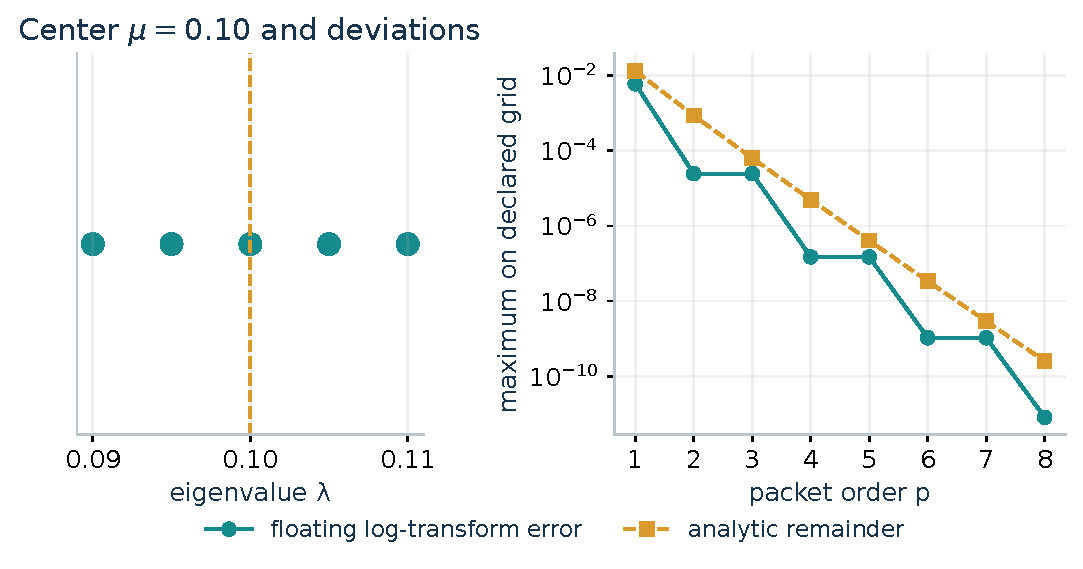
\includegraphics[width=\linewidth,height=3.1in,keepaspectratio]{figures/10_packet.pdf}\end{center}
{\small\color{navy}Centered storage and the declared-grid remainder ladder for one finite packet.}

\[M_{P,m}=\sum_{j\in P}(\lambda_j-\mu_P)^m,\quad\alpha_P(s)=\frac{2s}{1-2s\mu_P},\quad\rho_P(s)=|\alpha_P(s)|\max_{j\in P}|\lambda_j-\mu_P|.\]
\[\kappa_P(s)=-\frac{n_P}{2}\log(1-2s\mu_P)+\frac12\sum_{m=1}^{p}\frac{\alpha_P(s)^m M_{P,m}}m+R_{P,p}(s),\]
\[|R_{P,p}(s)|\le\frac{n_P}{2}\frac{\rho_P(s)^{p+1}}{(p+1)(1-\rho_P(s))}.\]
A packet contains nearby eigenvalues, their arithmetic mean $\mu_P$, and centered power sums $M_{P,m}$. Its first centered moment vanishes in exact arithmetic. Instead of substituting one surrogate eigenvalue or one surrogate distribution, the representation expands the packet contribution to the log transform.

Use a nonempty packet of positive coefficients, integer order $p\ge0$, and $\Re s<1/(2\lambda_{\max})$. The logarithm is the analytic principal branch on this transform domain. If $\rho_P(s)<1$, its power series gives the explicit remainder. The bound decreases geometrically when the radius ratio stays away from one.

The five-eigenvalue control uses $0.09,0.095,0.10,0.105,0.11$, a tilt of one, and 220 frequencies from zero to eighteen. The figure compares floating transform errors with the analytic remainder at orders one through eight. These computations illustrate the bound; they do not enclose library rounding.

\begin{tcolorbox}[colback=pale,colframe=teal,boxrule=.4pt,arc=2pt,left=7pt,right=7pt,top=5pt,bottom=5pt]\small\bfseries The local packet representation requires the transform domain, logarithm branch, and printed radius condition.\end{tcolorbox}
\vfill{\footnotesize\color{navy}\textbf{Source anchors.} K-COS source: Centered spectral packets / Centered packet expansion.}
\clearpage
{\small\bfseries\color{teal}11 \textperiodcentered{} Grid-dependent compilation}

{\LARGE\bfseries\color{navy}The query determines the useful packet\par}
\vspace{3pt}
\begin{center}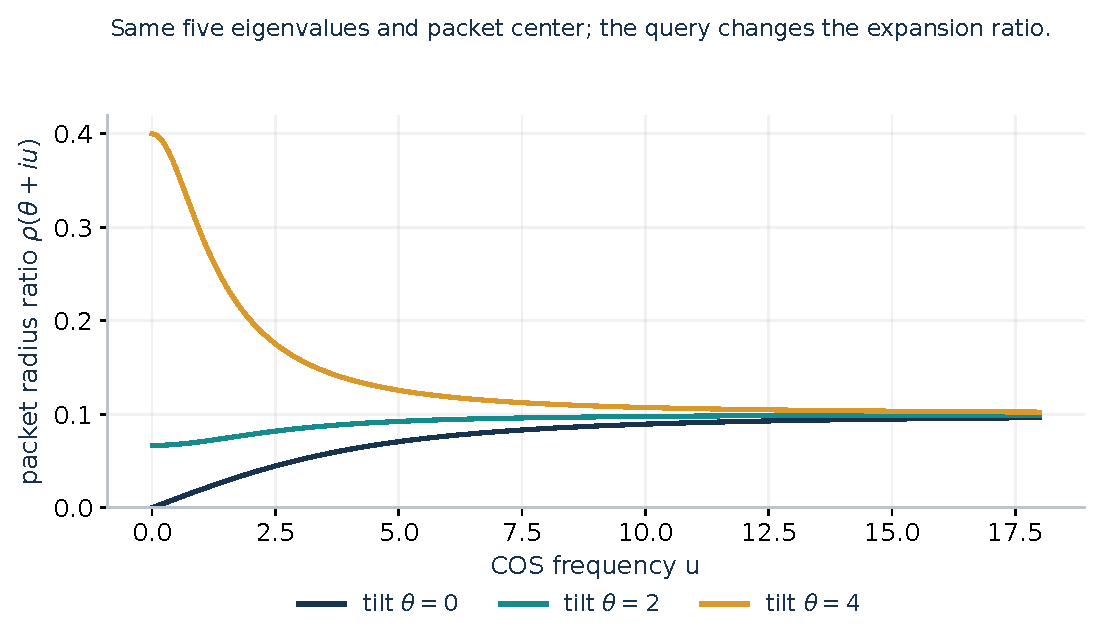
\includegraphics[width=\linewidth,height=3.1in,keepaspectratio]{figures/11_query_grid.pdf}\end{center}
{\small\color{navy}The same spectral packet has different expansion ratios at tilts zero, two, and four.}

\[s_k=\theta+i\frac{k\pi}{U},\qquad\rho_P(s_k)<1\quad\text{on every retained frequency}.\]
\[(\Lambda,q,\varepsilon)\longmapsto\mathcal P_{\Lambda,q,\varepsilon}.\]
A distance between eigenvalues is insufficient to decide whether a packet is useful. The expansion must be controlled at the actual complex arguments $s_k=\theta+i k\pi/U$ selected by the tail query. The tilt, support endpoint, and retained mode count all change that grid.

The figure holds the same five eigenvalues and packet center fixed while changing the tilt. Near the transform singularity the low-frequency radius can grow sharply. At high frequency the radius approaches the relative packet half-width. Neither effect is captured by inspecting raw eigenvalue spacing alone.

The compiled representation may retain large spikes exactly and packetize a smooth spectral bulk. Split a packet or raise its order when its propagated error exceeds budget. A plan can be reused only after checking that its stored conditions and grid remain applicable to the new request.

\begin{tcolorbox}[colback=pale,colframe=teal,boxrule=.4pt,arc=2pt,left=7pt,right=7pt,top=5pt,bottom=5pt]\small\bfseries The passport belongs to a spectrum, a query, and an accuracy contract, rather than to the spectrum alone.\end{tcolorbox}
\vfill{\footnotesize\color{navy}\textbf{Source anchors.} K-COS source: Centered spectral packets / Query dependence; Adaptive K-COS algorithm.}
\clearpage
{\small\bfseries\color{teal}12 \textperiodcentered{} Finite-window transform}

{\LARGE\bfseries\color{navy}Cosine inversion integrates a weighted tail\par}
\vspace{3pt}
\begin{center}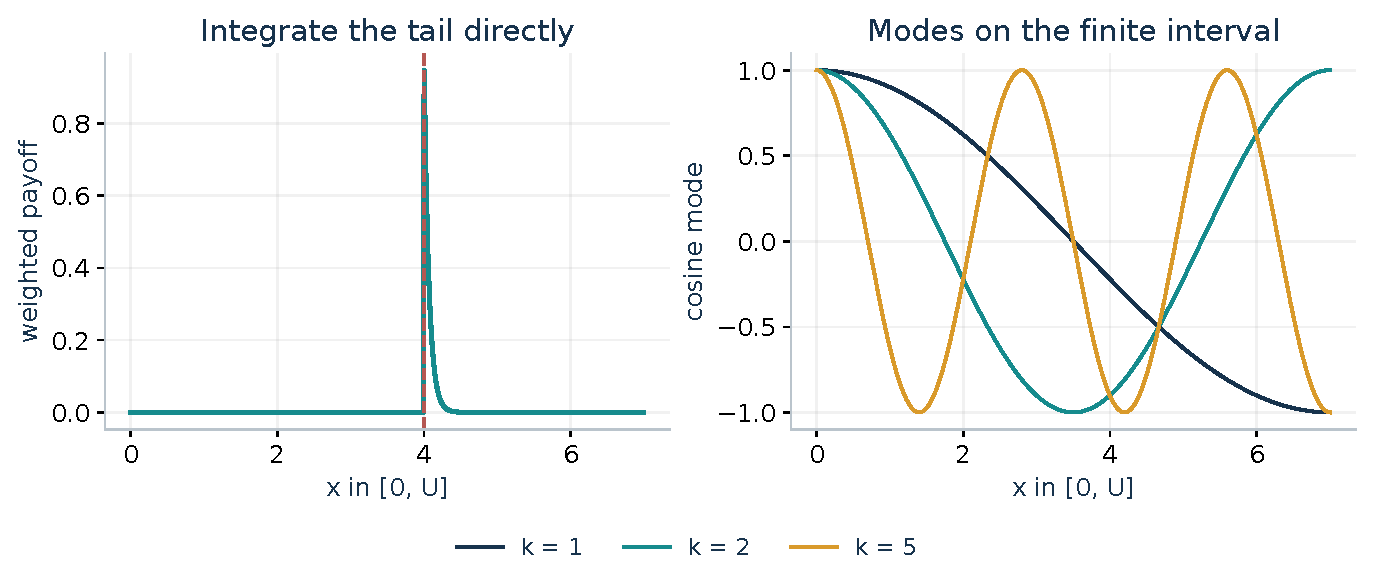
\includegraphics[width=\linewidth,height=3.1in,keepaspectratio]{figures/12_cos.pdf}\end{center}
{\small\color{navy}The weighted payoff and finite-interval basis have different roles. The prime gives half weight to mode zero.}

\[I_k=\int_q^Ue^{-\theta(x-q)}\cos(u_kx)\,dx=\Re\!\left[e^{iu_kq}\frac{1-e^{(-\theta+iu_k)(U-q)}}{\theta-iu_k}\right].\]
\[S_K=\frac2U\sum_{k=0}^{K-1}{}^{\prime}\, I_k\,\Re\,\phi_\theta(u_k),\qquad\phi_\theta(t)=e^{\kappa(\theta+it)-\kappa(\theta)}.\]
On a positive-support interval $[0,U]$, the cosine frequencies are $u_k=k\pi/U$. The payoff is zero below the threshold and decays exponentially above it. Integrating each cosine mode against that payoff gives an explicit coefficient.

The finite sum uses the tilted characteristic function rather than a CDF value close to one. Multiplying by the likelihood-ratio prefactor returns the original tail scale. This avoids subtracting two almost equal numbers, but it does not remove the need to bound discarded support and omitted modes.

The picture uses $q=4$, $U=7$, and $\theta=15$. It separates the payoff shape from three cosine modes. Correctness of the positive-support backend requires $q\ge0$ and $U>q$. The saddlepoint planner additionally selects upper-tail queries above the original mean.

\begin{tcolorbox}[colback=pale,colframe=teal,boxrule=.4pt,arc=2pt,left=7pt,right=7pt,top=5pt,bottom=5pt]\small\bfseries A finite-window, finite-mode transform is an intermediate quantity whose omitted contributions require bounds.\end{tcolorbox}
\vfill{\footnotesize\color{navy}\textbf{Source anchors.} Traditional paper: Directed-rounding deep-tail enclosure / Final enclosure theorem. K-COS source: Tilted COS tail functional.}
\clearpage
{\small\bfseries\color{teal}13 \textperiodcentered{} Omitted Fourier modes}

{\LARGE\bfseries\color{navy}Mode decay bounds the infinite remainder\par}
\vspace{3pt}
\begin{center}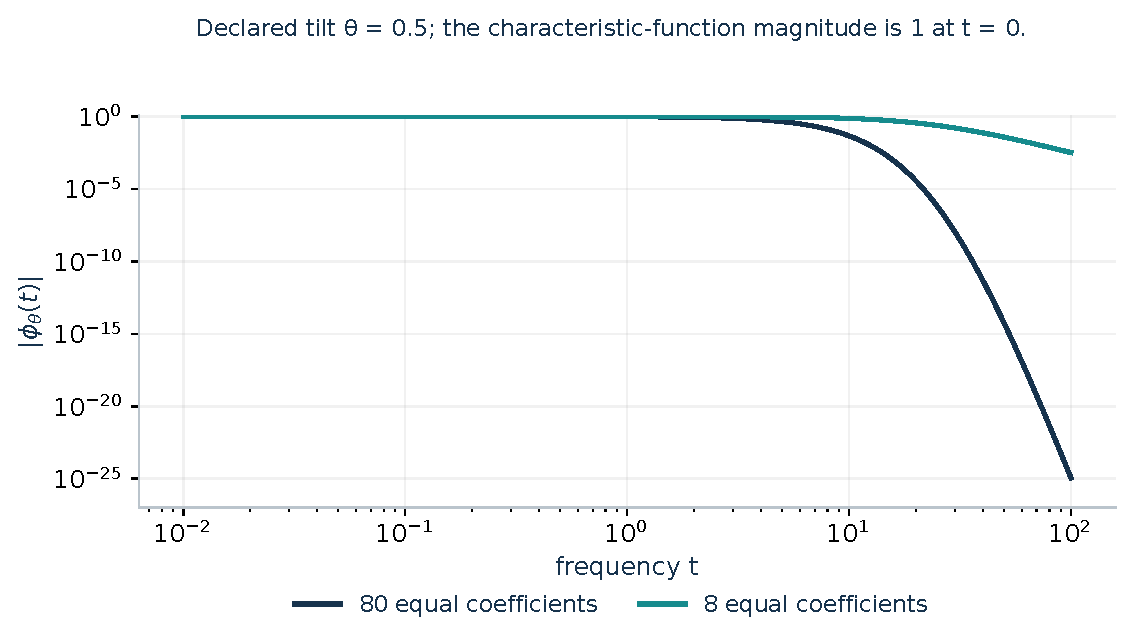
\includegraphics[width=\linewidth,height=3.1in,keepaspectratio]{figures/13_mode_decay.pdf}\end{center}
{\small\color{navy}Declared equal-coefficient controls illustrate why the number of active coefficients affects high-frequency decay.}

\[a_j=\frac{2\lambda_j}{1-2\theta\lambda_j},\quad|\phi_\theta(t)|=\prod_j(1+(a_jt)^2)^{-1/4}\le C_\theta t^{-r/2}.\]
\[E_{\rm series}\le\frac{2C_\theta}{U\theta}\left(\frac U\pi\right)^\nu\left[K^{-\nu}+\frac{K^{1-\nu}}{\nu-1}\right],\quad\nu=r/2>1.\]
The modulus of the normalized tilted characteristic function has a positive product formula. Its decay is controlled by the actual transformed coefficients. More active positive coefficients increase the asymptotic decay exponent.

The figure compares eight and eighty equal coefficients at the same admissible tilt. It evaluates the exact modulus formula in ordinary floating arithmetic. A rapidly falling curve is useful for choosing modes, but acceptance depends on a proved bound for the entire omitted series.

The rigorous interval backend uses a simple envelope $C_\theta t^{-r/2}$ and the payoff bound $|I_k|\le1/\theta$. Its resulting series bound requires $r>2$. The packetized analytic path has a sharper frequency-dependent decay-rate bound. Those are distinct formulas with distinct implementation scopes.

\begin{tcolorbox}[colback=pale,colframe=teal,boxrule=.4pt,arc=2pt,left=7pt,right=7pt,top=5pt,bottom=5pt]\small\bfseries The infinite-mode remainder is a mathematical tail of a series, separate from floating summation error.\end{tcolorbox}
\vfill{\footnotesize\color{navy}\textbf{Source anchors.} Traditional paper: Directed-rounding deep-tail enclosure / Rigorous infinite-mode control. K-COS source: Omitted COS-mode certificate.}
\clearpage
{\small\bfseries\color{teal}14 \textperiodcentered{} Analytic and arithmetic budgets}

{\LARGE\bfseries\color{navy}The error ledger keeps separate causes\par}
\vspace{3pt}
\begin{center}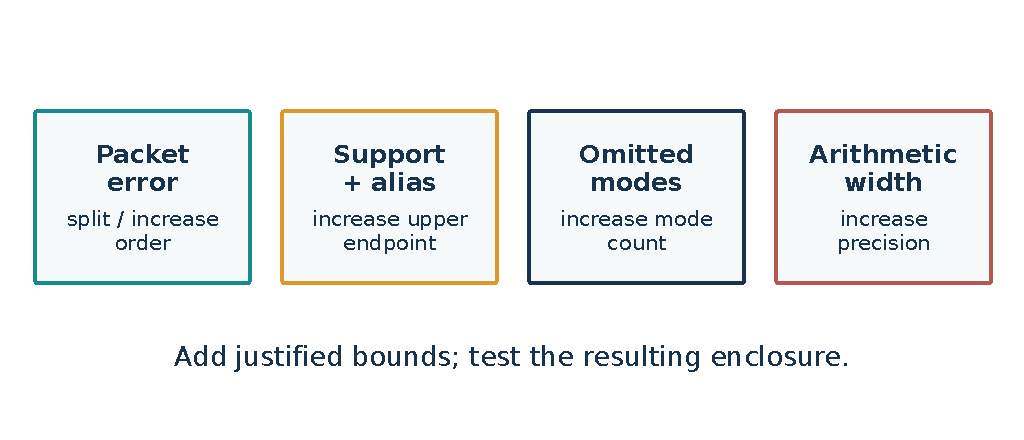
\includegraphics[width=\linewidth,height=3.1in,keepaspectratio]{figures/14_ledger.pdf}\end{center}
{\small\color{navy}Four causes of uncertainty and their natural controls. Every budget must be justified before acceptance.}

\[|p-\widehat p|\le E_{\rm packet}+E_{\rm support}+E_{\rm modes}\quad\text{(analytic packet path)}.\]
\[S_\theta(q)\in\boldsymbol S_K+[-E,E],\qquad E=E_{\rm support}+E_{\rm series}\quad\text{(exact-spectrum interval path)}.\]
Packet approximation changes the retained-grid transform. Support truncation and cosine periodization change the finite-window functional. Mode truncation removes infinitely many terms. These three mathematical approximation errors have different refinement controls and must be accounted for separately.

Directed-rounding arithmetic introduces a fourth quantity: the width of the computed interval for finite operations. That width is not a substitute for an analytic remainder. Conversely, an analytic bound does not automatically enclose the rounding of logarithms, exponentials, or summation.

For the exact-spectrum interval backend, no packet approximation is used. The finite transform interval is enlarged by support and series bounds, then passed through a positive logarithm and prefactor enclosure. Extending directed-rounding certification to the packet transform requires enclosing its moment construction and remainder propagation as well.

\begin{tcolorbox}[colback=pale,colframe=teal,boxrule=.4pt,arc=2pt,left=7pt,right=7pt,top=5pt,bottom=5pt]\small\bfseries Name the uncertainty before refining it. The same scalar tolerance can hide different unresolved causes.\end{tcolorbox}
\vfill{\footnotesize\color{navy}\textbf{Source anchors.} Traditional paper: Directed-rounding deep-tail enclosure; Accuracy-driven certification. K-COS source: Combined analytic certificate / Certificate boundary.}
\clearpage
{\small\bfseries\color{teal}15 \textperiodcentered{} Requested accuracy}

{\LARGE\bfseries\color{navy}Acceptance is a logarithmic interval test\par}
\vspace{3pt}
\begin{center}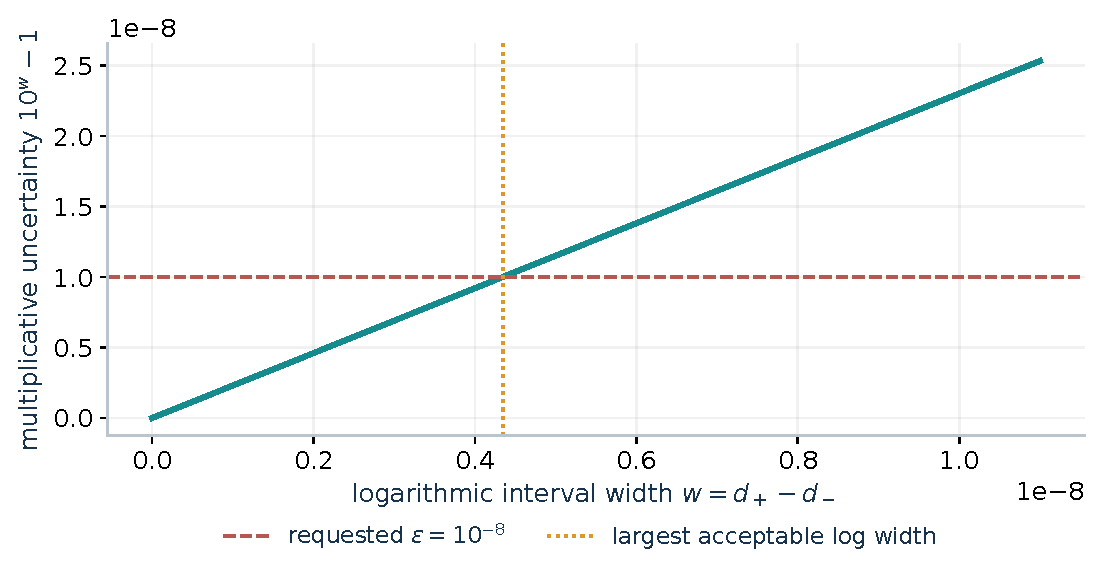
\includegraphics[width=\linewidth,height=3.1in,keepaspectratio]{figures/15_acceptance.pdf}\end{center}
{\small\color{navy}An illustrative tolerance of $10^{-8}$ determines the permitted log width; the plotted curve is numerical.}

\[\log_{10}p\in[d_-,d_+],\quad w=d_+-d_-,\quad\frac{p_+}{p_-}-1=\operatorname{expm1}(\log(10)w).\]
\[\operatorname{expm1}(\log(10)w)\le\varepsilon\quad\Longrightarrow\quad\text{requested enclosure width is met}.\]
A positive probability enclosure can be stored on a logarithmic scale even when its endpoints are below ordinary floating-point range. If $d_-$ and $d_+$ enclose $\log_{10}p$, the width determines the maximum multiplicative uncertainty.

For validated acceptance, compute the width and $\operatorname{expm1}(\log(10)w)$ with directed interval arithmetic. Compare the ratio interval\textquotesingle s upper endpoint to the exact tolerance enclosure\textquotesingle s lower endpoint. Preserve the literal outer endpoints throughout parsing and conversion. High precision alone does not prove this decision.

The controller returns an accepted result only after the full enclosure passes the requested tolerance. An unresolved positive lower bound, invalid transform domain, inadequate mode budget, or exhausted precision budget must produce a failure status. A point estimate can still be informative, but it cannot be relabeled as an accepted enclosure.

\begin{tcolorbox}[colback=pale,colframe=teal,boxrule=.4pt,arc=2pt,left=7pt,right=7pt,top=5pt,bottom=5pt]\small\bfseries The decision logic and input semantics are part of certification, just as the transform arithmetic is.\end{tcolorbox}
\vfill{\footnotesize\color{navy}\textbf{Source anchors.} Traditional paper: Accuracy-driven certification / Fail-closed behavior; Acceptance arithmetic is itself high precision.}
\clearpage
{\small\bfseries\color{teal}16 \textperiodcentered{} Independent control family}

{\LARGE\bfseries\color{navy}An exact-law control reaches deep logarithms\par}
\vspace{3pt}
\begin{center}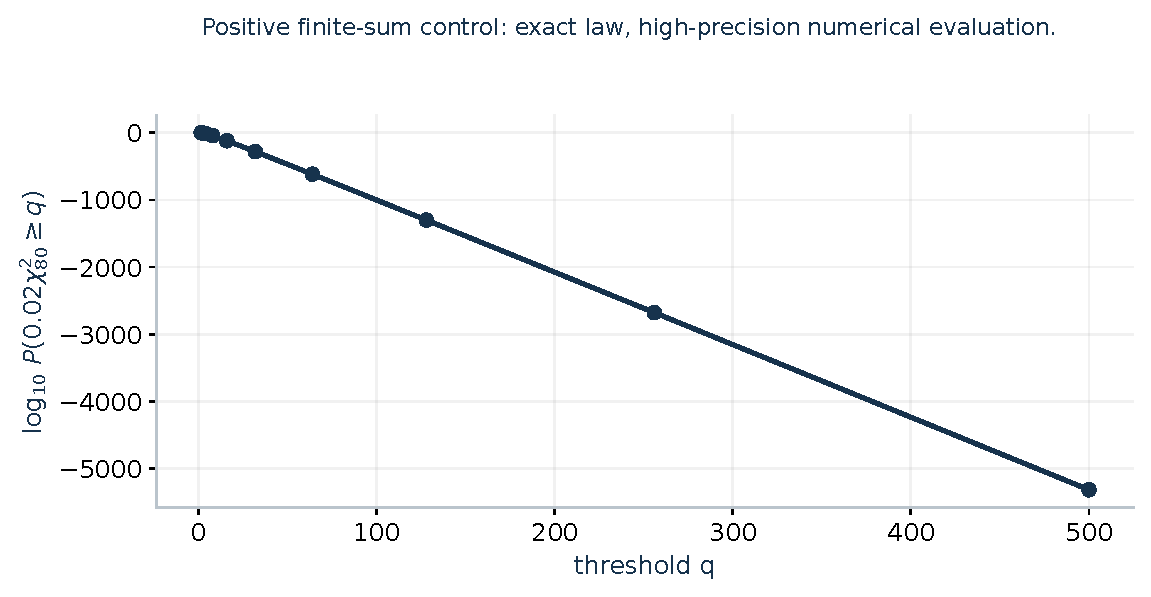
\includegraphics[width=\linewidth,height=3.1in,keepaspectratio]{figures/16_exact_control.pdf}\end{center}
{\small\color{navy}An independently evaluable exact-law family. The plot is regenerated from a positive finite sum in decimal arithmetic.}

\[z=q/0.04,\qquad P(Q\ge q)=e^{-z}\sum_{k=0}^{39}\frac{z^k}{k!}.\]
\[\log_{10}P(Q\ge q)=\frac{-z+\log\!\left(\sum_{k=0}^{39}z^k/k!\right)}{\log(10)}.\]
For an even-degree chi-square variable, the upper tail has a finite positive-sum formula. The control $Q=0.02\chi^2_{80}$ is a gamma law of integer shape forty and scale $0.04$. Its survival probability can therefore be evaluated independently of cosine inversion.

The curve computes the logarithm first. At thresholds from $1.6$ through $500$, it evaluates the finite sum with ninety decimal digits and plots its logarithm. The exact law supplies the formula; the numeric points are high-precision evaluations rather than directed-rounding enclosures.

This control can distinguish a transform error from a reference error without relying on another COS run. Its equal-coefficient structure also means that one packet can represent the spectrum exactly. Success on this family does not establish equal performance for heterogeneous spectra, signed laws, or every matrix-to-spectrum bridge.

\begin{tcolorbox}[colback=pale,colframe=teal,boxrule=.4pt,arc=2pt,left=7pt,right=7pt,top=5pt,bottom=5pt]\small\bfseries Choose a reference with a different mathematical route. Report its arithmetic scope alongside the result.\end{tcolorbox}
\vfill{\footnotesize\color{navy}\textbf{Source anchors.} Traditional paper: Directed-rounding deep-tail enclosure / Independent exact interval control through 1e-5000.}
\clearpage
{\small\bfseries\color{teal}17 \textperiodcentered{} Publication and evidence map}

{\LARGE\bfseries\color{navy}Read the three companions with their scopes\par}
\vspace{3pt}
\vspace{5pt}\begin{center}\small\renewcommand{\arraystretch}{1.3}\begin{tabular}{@{}>{\raggedright\arraybackslash}p{.25\linewidth}>{\raggedright\arraybackslash}p{.33\linewidth}>{\raggedright\arraybackslash}p{.36\linewidth}@{}}\toprule
Representation layer & Evidence to inspect & Scope to preserve\\
\midrule
Block / projector algebra & Exact identities; selected Lean sources & All required hypotheses and finite dimensions\\
Computed spectrum & Validated matrix-to-spectrum bridge & Input semantics; residual and rounding enclosures\\
Spectral packet transform & Analytic remainders; executable checks & Complex-grid radius; arithmetic error\\
Positive exact-spectrum tail & Directed-rounding interval; analytic bounds & Admissible tilt; positive support; active rank\\
Controller decision & Enclosure-width test; precision and parsing tests & Requested tolerance; explicit failure status\\
\bottomrule\end{tabular}\end{center}
\[\text{matrix input}\ \longrightarrow\ \text{spectral enclosure}\ \longrightarrow\ \text{tail enclosure}\ \longrightarrow\ \text{accepted width}.\]
The traditional paper explains the operator identities, propagation bounds, residual structure, packet construction, and probability enclosures. This visual companion makes those mechanisms inspectable through small declared cases. The Lean companion identifies exactly which algebraic or analytic statements are represented by its source files and what the checked build establishes.

A Lean proof of block matrix algebra does not automatically certify a Python eigensolver, a decimal parser, or a transcendental interval library. A directed-rounding tail computation for exact supplied coefficients does not automatically certify coefficients computed by an unverified SVD. Each interface needs its own evidence.

The final release preserves executable sources and verification records. Rebuild the figures with the supplied script, inspect the finite control record, and compare the formalization guide with its checked sources. All illustrations use declared controls, and no empirical timing or production tail claim is introduced by this guide.

\begin{tcolorbox}[colback=pale,colframe=teal,boxrule=.4pt,arc=2pt,left=7pt,right=7pt,top=5pt,bottom=5pt]\small\bfseries A complete result carries its assumptions, representation semantics, numerical enclosure, and formal scope.\end{tcolorbox}
\vfill{\footnotesize\color{navy}\textbf{Source anchors.} Traditional paper: Guarantee boundary; Verified matrix-to-spectrum bridge / Scalability boundary; Reproducibility and formalization sections. Lean companion: formalization inventory.}
\end{document}
